\documentclass[10pt,a4paper,openany]{book}
\usepackage[spanish]{babel}
\usepackage[version=3]{mhchem} % Package for chemical equation typesetting
\usepackage{siunitx} % Provides the \SI{}{} and \si{} command for typesetting SI units
\usepackage{graphicx} % Required for the inclusion of images
\usepackage{natbib} % Required to change bibliography style to APA
\usepackage{amsmath} % Required for some math elements 
\usepackage{multirow} % for tables
\usepackage{longtable} % for long tables
\usepackage[left=1.5cm,right=1.5cm,top=2.54cm,bottom=2.54cm]{geometry}
\setlength\parindent{0pt} % Removes all indentation from paragraphs
\graphicspath{{./img/}}
%\renewcommand{\labelenumi}{\alph{enumi}.} % Make numbering in the enumerate environment by letter rather 
%----------------------------------------------------------------------------------------
%	DOCUMENT HEADER
%----------------------------------------------------------------------------------------
\def\BibTeX{{\rm B\kern-.05em{\sc i\kern-.025em b}\kern-.08em
    T\kern-.1667em\lower.7ex\hbox{E}\kern-.125emX}}
	\graphicspath{{./img/}}
	\usepackage{fancyhdr} % Headers and footers
	\pagestyle{fancy} % All pages have headers and footers
	\fancyhead[L]{Fac. de Ingenier\'ia y Ciencia}
	\fancyhead[C]{2020 - 2} % Custom header text
	%\fancyfoot[RO,LE]{\thepage} % Custom footer text
	\fancyhead[R]{
\includegraphics[width=0.14\linewidth]{Logo-PUJ-Negro}\vspace{-0.2cm}}
	\fancypagestyle{firstpage}{%
	\fancyhead[L]{Fac. de Ingenier\'ia y Ciencia}
	\fancyhead[C]{} % Custom header text
	\fancyhead[R]{
\includegraphics[width=0.14\linewidth]{Logo-PUJ-Negro}\vspace{-0.2cm}}
}
%----------------------------------------------------------------------------------------
%	DOCUMENT
%----------------------------------------------------------------------------------------
\begin{document}
\begin{titlepage}
	\begin{center}
		{\Large \textbf{LÍNEAS DE PRODUCTOS DE SOFTWARE}}\\
		\vspace{3cm}
		{\Large \textbf{LÍNEA TALLERES VIRTUALES}}\\
		\vspace{3cm}
		{\large \today}\\
		\vspace{3cm}
		{\large \textbf{Óscar Fernando Calero Mayor}}\\
		{\large \textbf{William Andrey Garzón Bohóquez}}\\
		{\large \textbf{Dario Leonardo Narváez Jácome}}\\
		\vspace{1cm}
		{\large Pontificia Universidad Javeriana de Cali}\\
		{\large Facultad de Ingeniería y Ciencias}\\
		\begin{figure}[h]
			\centering
			
\includegraphics[scale=0.8]{logo}
		\end{figure}
	\end{center} 
\end{titlepage}

\tableofcontents

%----------------------------------------------------------------------------------------
%	1 Definición del alcance
%----------------------------------------------------------------------------------------
\chapter{Definición del alcance}
%----------------------------------------------------------------------------------------
%	1.1. Estudio del mercado y de factibilidad
%----------------------------------------------------------------------------------------
\section{Estudio del mercado y de factibilidad}
%----------------------------------------------------------------------------------------
%	1.1.1 Análisis de problema y las oportunidades
%----------------------------------------------------------------------------------------
\subsection{Análisis de problema y las oportunidades}

Con la revolución 4.0 muchas compañías han optado por generar nuevos servicios tecnológicos para brindar mejor servicio a sus clientes y dar un servicio más personalizado a las necesidades de los clientes. Existen muchas compañías como pymes o microempresa que no poseen el recurso para acceder al desarrollo de estos servicios tecnológicos y que les permitan mantenerse competitivos en este mercado cambiante de tecnología. Dentro de estas compañías se encuentran los talleres de automóviles que poseen mucha variedad por servicios y por tamaño es por esta razón que se tiene una oportunidad para crear un LP que cubra la necesidad de cada tipo de taller o servicios que ofrezcan.

\subsection{Entender hacia dónde se quiere ir}

El mercado de ventas de vehículos en un mercado que se mantiene en crecimiento después de una caída por la cuarentena ocurrida por el COVID esto genera en cierto modo que se vea afectado positivamente el mercado de servicios de taller puesto que al tener más parque automotor en circulación eso genera un crecimiento en las compañías de talleres de vehículos ya sean las compañías existentes que adapten nuevos servicios a ofrecer o que se creen nuevos talleres para cubrir la demanda. Por esta razón se hace necesario herramientas de software para estos talleres que se adapten al portafolio de servicios que ofrecen y rápidamente por que es un cliente de un taller debe ser atendido en mayor brevedad posible. Por este motivo se propone utilizar un paradigma de desarrollo de software basado en líneas de productos LP que permita adaptarse a las necesidades de cada tipo de taller.

\subsection{Determinar el segmento del mercado}

Para segmentar el mercado utilizaremos las variables geográficas, demográficas, legales y socioeconómicas. Para las variables geográficas y legales porque existe leyes y reglamentaciones a la cual se debe regir estos tipos de negocios en cada país y más específicos para esta LP al país Colombia donde existen entidades regulatorias que protegen al consumidor como por ejemplo Superintendencia de industria y comercial y los talleres deben regirse con esta normativa para no incurrir en sanciones.
Por otro lado, la variable demográfica por que se busca brincar herramienta para gestionar talleres, pero se enfocará en los propietarios de talleres menores a 40 años ya que es posible que se adopten más fácil nuevas tecnologías que beneficien sus negocios.
Y finalmente la variable socioeconómica por que estará enfocado en negocios micro y pymes para brincar una herramienta que les permita ser más competitivos.


\subsubsection{Requisitos funcionales}

\begin{enumerate}
\item El sistema debe permitir a los clientes registrarse utilizando Facebook o Google.
\item El sistema debe tener un sistema de autenticación a los usuarios del taller.
\item El sistema tendrá un catálogo de servicios que podrá ofrecer por parte del taller.
\item El sistema tendrá gestión de los horarios disponibles por servicios.
\item El sistema permitirá buscar por palabras claves, precios y disponibilidad al cliente servicios que ofrecen el taller.
\item El sistema permite al cliente pagar por algunos servicios vía electrónica: tarjeta de crédito o tarjeta débito.
\item El sistema de pago debe utilizar pasarela de pago como PayU en Colombia.
\item El sistema debe permitir al cliente cancelar la reserva.
\item El sistema debe permitir recuperar al usuario.
\item El sistema debe tener un componente de historia de servicios solicitados.
\item El sistema debe permitir generar facturación electrónica a los clientes
\end{enumerate}


\subsubsection{Requisitos no funcionales}

\begin{enumerate}
\item El sistema debe ser responsivo y adaptarse a Computadores, Tablet o Móviles
\item El sistema debe aplicar la reglamentación colombiana para este tipo de servicios
\item La información financiera de los clientes debe manejarse de forma segura
\item La información de los clientes debe respectar las leyes de habeas data
\item El sistema debe ser de fácil mantenibilidad
\item El sistema debe tener disponibilidad
\item El sistema debe ser pensando en usabilidad
\item El sistema debe dar respuesta a cualquier petición con un tiempo menor a 10 seg
\end{enumerate}

\subsection{Identificar las posibles soluciones y sus alcances}
 
¿Qué productos tendrá la LP?\\
Sistemas de tienda de servicios online para talleres del sector automotriz por ejemplo 1) Taller que ofrece mecánica y lavado, 2) Taller que ofrece mecánica, lavado y pintura y 3) Taller que ofrece mecánica, lavado, pintura y Audio.\\\\
 ¿Cuál es su mercado?\\
Talleres de automóviles de Valle del Cauca – Colombia.\\\\
¿Cuándo serán lanzados?\\
Una vez terminado análisis, diseño e implementación de la LP y con sus pruebas correspondientes\\
¿Cuál será el subdominio de la LP?\\
El dominio serán comercio electrónico y el subdominio comercio electrónico de servicios de talleres de automóviles.\\\\
¿Qué ventajas y desventajas ofrece este subdominio?\\
El comercio electrónico en Colombia ha tenido un crecimiento ya que existe una sociedad más digital y dispuesta a comprar online en el año 2019 tuvo un crecimiento de 27\% con respecto al 2018 y colocando a Colombia en el cuarto mercado de la región moviendo 7.6 mil millones USD y con la posibilidad para el 2021 ocupar el tercer puesto en mercado electrónico desplazando Argentina. Por otro lado, el mercado de ventas de vehículos está retomando participación después de abril del 2020 por la cuarentena y con un crecimiento eso generará más parque automotor y más demanda de servicios para los talleres automotrices.\\\\
¿Qué características tendrá la LP?\\
En cuanto a requisitos funcionales un comercio electrónico se basa en la información que se presenta y que sea fácil consultar por otro lado está LP debido a que es un comercio electrónico enfocado en oferta y demanda de servicios de talleres de automóviles debe permitir consultar atributos como precio, disponibilidad, productos entre otros, permitiéndole a los registrar usuarios tanto internos como externos. Igualmente debe permitir a los clientes reservar alguno de los servicios ofrecidos por el taller   y como una facilidad para el cliente y el taller que se puede pagar por el servicio con anterioridad por medio electrónico o pagar en el taller.\\
En cuanto a los requisitos no funcionales debe ser portable ósea funcionar el cualquier dispositivos tabletas, móviles y pc. También se debe tener alta disponibilidad ya que este mercado requiere atención muy rápida al cliente debido a que normalmente cuando un cliente requiere un servicio de taller es por que lo necesita de manera urgente y que el sitio no esté disponible puede ocasionar que pierda un cliente.\\
Por último, como da la posibilidad de pagar por medio electrónico se debe ofrecer todos los estándares de seguridad que protejan a los clientes y al taller de fraudes electrónicos.\\\\
 
¿Qué tipos de productos tendrá la LP y que variaciones?\\
Los productos de la línea sería de tipo software y las variaciones que tendrá depende del taller y los servicios que ofrecen cada uno de ellos por ejemplo alguno taller tendrán el módulo de gestión de lavado de vehículo, módulo de gestión de mecánica, módulo de gestión pintura, módulo de gestión de audio, módulo para gestión de horarios y módulo para gestión de lista de precios y con la posibilidad que tenga todos o alguno de estos módulos.\\\\
¿Cuáles son las oportunidades y riesgo que presentan las variaciones de la LP?\\
Una oportunidad es atraer nuevos clientes que necesitan alguno de los servicios que ofrece cada módulo, otra oportunidad es fidelizar a los clientes del taller al ofrecer un mejor servicio y de fácil acceso. Para el módulo de pagos online tendrá una oportunidad de generar mayor satisfacción de los clientes por que ahorra tiempo en realizar el servicio un riesgo problemas en los pagos de los clientes. Un riesgo podría ocurrir por tener que pedir a los clientes de los talleres registrarse eso puede generar que no ingresen y se pierda un posible prospecto o cliente. Y finalmente una gran oportunidad es poder difundir de manera masiva los servicios del taller y permitir a los clientes tener un contacto más personalizado con el taller.\\\\
¿Cuáles componentes reutilizables se incluirán en la LP?\\
Dado que este comercio electrónico ofrece servicios de un taller de automóviles es necesario que existe por lo menos un módulo del servicio que se ofrecen:  mecánica, pintura, lavado y Audio y el módulo de administración del sistema ya con esta restricción se podría consultar los servicios que ofrece el taller, pero aun no se podría pagar en línea o conocer precios de estos y finalmente el módulo de horario para manejar el tiempo de disponibilidad del taller para reservar del cliente.\\\\
¿Cuáles de ellos puedo realmente implementar con los recursos disponibles y el estado actual de la empresa?\\
Para el ejercicio se asume que se tiene todos los recursos disponibles para cumplir la implementación.\\\\
¿con qué clase de elementos reutilizables cuento actualmente (componentes o documentación existentes)?\\
Debido a que es una oportunidad para un nuevo proyecto no cuentan actualmente con ningún componente o documentación para reutilizar.\\ \cite{url1} \cite{url2}


\subsection{Evaluación}

\textbf{Identificación de riesgos}\\
En la Tabla~\ref{table:t7}, se presenta un matriz de riesgos para una implementación de una LP para un comercio electrónico para ofrecer servicios de talleres de automóviles según su probabilidad de ocurrencia, impacto de riesgo y las acciones que lo disminuyen.

\begin{table}[htbp]
\centering
\begin{tabular}{|p{3cm}|p{4cm}|p{2cm}|p{2cm}|p{4cm}|} \hline
Alternativa & Riesgo & Ocurrencia & Impacto & Acciones atenuante \\ \hline
\multirow{4}{3cm}{Implementación de una línea de productos en comercio electrónico para servicios talleres de automóviles} & Que los módulo reutilizables no se puedan acoplar de manera correcta
 & Baja & Alto & Se deben hacer un plan de pruebas para cada módulo
\\
\cline{2-5} & Que la implementación de cada uno de los componentes no se pueda realizar en el tiempo previsto & Media & Alto & Se debe hacer una implementación iterativa\\ 
\cline{2-5} & Que el cliente no queda satisfecho con el software solicitado
 & Media & Alto & Se debe realizar una buena educción de requisitos\\ 
\cline{2-5} & Que existan funcionalidades que no sean necesarias o que falten funcionalidades necesarias para cumplir el servicio del cliente & Media & Alto & Se debe realizar una buena educción de requisitos\\ \hline
\end{tabular}
\caption{Matriz de riesgos}
\label{table:t7}
\end{table}


Finalmente se detallan todos los problemas que pueden ocurrir en la etapa de implementación para una línea de producto en comercios electrónicos para servicios de taller de automóviles en la Tabla~\ref{table:t8}:

\begin{table}[htbp]
\centering
\begin{tabular}{|p{4cm}|p{4cm}|p{2cm}|p{4cm}|} \hline
Alternativa & Descripción del problema & Prioridad del problema & Acciones para su resolución \\ \hline
\multirow{2}{3cm}{Implementación de una línea de productos en comercio electrónico para servicios talleres de automóviles} & Necesita autorización de generación & 3 & Presentar beneficios en tiempo y costos a largo plazo de implementar un LP \\
\cline{2-4} & Falta de conocimiento en implementar un LP & 4 & Se hace necesario contratar un líder de proyecto que conozca de implementación de LP\\ 
\cline{2-4} & Se requiere mayor nivel de inversión para iniciar una LP & 2 & Plantear costos y gastos necesarios para implementar LP vs Beneficios obtenidos a largo plaz\\  \hline
\end{tabular}
\caption{Posibles problemas}
\label{table:t8}
\end{table}


%----------------------------------------------------------------------------------------
%	1.2. Análisis de inversiones costos y rentabilidad
%----------------------------------------------------------------------------------------
\section{Análisis de inversiones costos y rentabilidad}

Ya que el equipo no cuenta con un musculo de inversión grande para iniciar con la línea de productos, decidimos implementar la estrategia de desarrollo incremental, con el fin de llegar a elaborar una gran cantidad de productos los valores aquí mostrados fueron obtenidos a partir de juicio de experto\\

El costo total de una LPS se descompone en costos fijos y costos variables como lo muestra la ecuación (\ref{eqn:eqn1}), donde:\\ CFlps corresponde a los costos fijos \\ CVlps corresponde a los costos variables.

\begin{equation}
C_{TotalLPS} = (CF_{LPS} + CV_{LPS})
\label{eqn:eqn1}
\end{equation}

los costos fijos de los productos a nivel operativo se pueden expresar mediante la ecuación (\ref{eqn:eqn2}), donde: \\
  CModDown son los costos de modelar el dominio \\
  CCOnfigProd corresponde a los costos de configuración de los productos\\
  CCPlatSoft se refiere a los costos del desarrollo de la plataforma \\
  CCDefComp equivale a los costos de definición \\
  CCConcepProd se trata de los costos de conseptializacion\\
\begin{equation}
CF_{ProdNivelOp} = C_{ModDown} + C_{COnfigProd} + C_{CPlatSoft} + C_{CDefComp} + C_{CConcepProd}  
\label{eqn:eqn2}
\end{equation}


La Tabla~\ref{table:t1} mustra un calculo estimado de los costos fijos (CFProdNivelOp)
 
\begin{table}[htbp]
\centering
\begin{tabular}{|c|c|c|c|p{2.5cm}|p{2.5cm}|} \hline
 Dato & Valor(\$)/h & Esfuerzo[LPS] (h) & Total(\$)[LPS] & Esfuerzo [Tradicional] (h) & Total(\$) [Tradicional]\\[0.5ex] \hline
 CModDom     & 20000 & 40  & 800000   & 0   & 0 \\[0.5ex] \hline
 CConfigProd & 25000 & 80  & 2000000  & 50  & 1250000 \\[0.5ex] \hline
 CPlatSoft   & 30000 & 384 & 11520000 & 300 & 9000000 \\[0.5ex] \hline
 CDefComp    & 20000 & 32  & 640000   & 16  & 320000  \\[0.5ex] \hline
 CConcepProd & 18000 & 40  & 720000   & 0   & 0       \\[0.5ex] \hline
 TOTAL &  &  & 15680000 & & 10570000\\[0.5ex] \hline
\end{tabular}
\caption{Costos Fijos}
\label{table:t1}
\end{table}

En la ecuación (\ref{eqn:eqn3}) CVLPS, corresponde al costo variable de la LPS. Este costo corresponde a los costos variables de los productos de nivel operativo.

\begin{equation}
CV_{LPS} = CV_{ProdNivelOp}  
\label{eqn:eqn3}
\end{equation}

\begin{equation}
CV_{ProdNivelOp} =  C_{DerivProd} 
\label{eqn:eqn4}
\end{equation}

\begin{equation}
C_{DerivProd} = C_{ConsepPro}  +  C_{UtilizaionComp}
\label{eqn:eqn5}
\end{equation}

Los costos de conceptualización de los productos CConcepProd constituyen los costos fijos de la derivación de productos, y en tanto que costos fijos, ya fueron incluídos en los costos fijos de los productos del nivel operativo por tanto la ecuación (\ref{eqn:eqn3})  se convierte en:

\begin{equation}
CV_{LPS} = C_{UtilizaionComp} 
\label{eqn:eqn6}
\end{equation}

Los costos de utilización de los componentes en la ecuación (\ref{eqn:eqn6}) están dados por la ecuación (\ref{eqn:eqn7}) donde:\\
NpNo es el número total de productos de nivel operativo de la LPS.\\
NCompProdNop es el número total de componentes del producto p de nivel operativo.\\
CConstruccionComp j,p son los costos de construcción (costos variables) del componente j, utilizado en el producto p.\\
NumProdUsanCompj es el número de productos de nivel operativo que utilizan el componente j.\\

\begin{equation}
C_{UtilizaionComp} = \sum_{p=1}NpNo \sum_{j=1}N_{CompProdNOp}\left(\frac{C_{ContruccionComp}}{NumProdUsanComp}\right)
\label{eqn:eqn7}
\end{equation}

\begin{quote}Para determinar los costos de la utilización de componentes, los expertos estiman el grado de utilización esperado para cada componente utilizable en los productos de nivel operativo, luego dividen los costos de construcción de cada componente por su grado de utilización.\cite{8048908}, para este caso o veremos los calculos en la Tabla~\ref{table:t2}.\end{quote}


\begin{table}[htbp]
\centering
\begin{tabular}{|c|c|c|} \hline
 Dato & Producto 1  & Producto 2 \\[0.5ex] \hline
 NCompProdNop      &  12 & 16  \\[0.5ex] \hline
 CConstruccionComp &  0  & 3840000  \\[0.5ex] \hline
 NumProdUsanCompj  &  1  & 2 \\[0.5ex] \hline
 CVProdNivelOp     &  0  &  1920000 \\[0.5ex] \hline
\end{tabular}
\caption{Costos Variables}
\label{table:t2}
\end{table}

Ahora calcularemos nuestro ROI punto de equilibro para estimar cuantos productos tenemos que vender para obtener el retorno de la inversion.

\begin{table}[htbp]
\centering
\begin{tabular}{|c|c|c|c|c|c|} \hline
 Caso & Producto 1  & Producto 2 & Producto 3 & Producto 4 & Producto 5\\[0.5ex] \hline
 Sin reutilizacion  & 10570000 & 21140000 & 42280000  & 84560000  & 169120000 \\[0.5ex] \hline
 Usando LPS         & 15680000 & 17600000 & 19520000  & 21440000  & 23360000 \\[0.5ex] \hline
 Ahorro con LPS     & 5110000  & 3540000  & 22760000  & 63120000  & 145760000 \\[0.5ex] \hline
 ROI                & -0,18    & 0.13     &  0,82     & 2,28      & 5,27 \\[0.5ex] \hline
 
\end{tabular}
\caption{Calculo del ROI}
\label{table:t3}
\end{table}


La Figura~\ref{fig:grf1} muestra los datos obtenido en la Tabla~\ref{table:t3} que compara los costos para desarrollar n productos de nivel operativo bajo enfoque tradicional versus LPS

\vspace{18cm}

\begin{figure}[h]
	\centering
	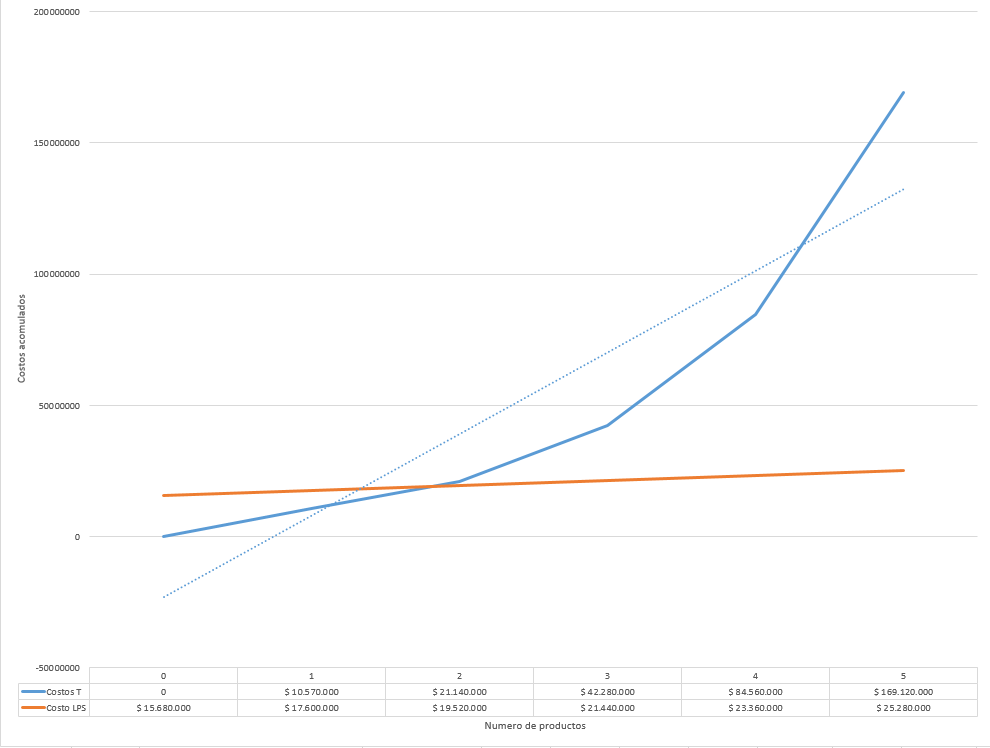
\includegraphics[width=1\textwidth]{grf1}
	\caption{Costos, enfoque tradicional versus LPS}
	\label{fig:grf1}
\end{figure} 

En conclusión, podemos ver que la rentabilidad de la línea de productos nos ofrece una rentabilidad positiva a partir del segundo producto vendido ya que la inversión inicial es de 15’680.000 COP y esta es recuperada con la venta del segundo producto, el cual se estima tiene unos costos variables de 1’920.000 COP y se vende a 17’600.000 COP produciendo una ganancia de 15’680.000 COP. 


%----------------------------------------------------------------------------------------
%	1.3. Análisis interno
%----------------------------------------------------------------------------------------
\section{Análisis interno}

\begin{longtable}{|c|p{8cm}|p{4cm}|} \hline
 Nombre & Habilildades  & Área de Conocimiento \\[0.5ex] \hline
 Oscar & PHP, Angular, JavaScript, Postgres, Kotlin   & Automotriz, Financiero \\[0.5ex] \hline
 William & Java, Angular, Python, JavaScript ,Spring MVC, BOOT, SECURITY, JSP, HTML, CSS, BOOTSTRAP, Thymeleaf, Hibernatem, SQL, WebService REST, SOAP   & Financiero, Bancario \\[0.5ex] \hline
 Dario & Java/Groovy, Angular   & Expedición Documentos Civiles, Domicilios \\[0.5ex] \hline
\caption{Análisis interno}
\label{table:t4}
\end{longtable}

\vspace{4cm}
%----------------------------------------------------------------------------------------
%	1.4. Definición del catálogo del producto
%----------------------------------------------------------------------------------------
\section{Definición del catálogo del producto}


\begin{table}[htbp]
\centering
\begin{tabular}{|p{5cm}|p{3cm}|p{3cm}|p{3cm}|} \hline
	& \textbf{Básico:} Gestión de servicios por BD  
	& \textbf{Profesional:} Gestión de servicios por Frontend(carga excel)  
	& \textbf{Experto:} Personalización de servicios por Frontend(formulario \\[0.5ex] \hline
Ingreso Anual$<$ \$1.131.000.000	                & TallerVirtual1  &  &  \\[0.5ex] \hline
\$1.131.000.000$<$ Ingreso Anual$<$ \$4.523.000.000	&   & TallerVirtual2 &  \\[0.5ex] \hline
Ingreso Anual $>$ \$4.523.000.000	                &   &  & TallerVirtual3 \\[0.5ex] \hline

\end{tabular}
\caption{Tabla de Segmentos 1}
\label{table:t5}
\end{table}

¿Quiénes son los principales actores de la industria?
\begin{itemize}
	\item Montallantas
	\item Lavado de autos
	\item Talleres Automotrices
	\item Pintura Automotriz
\end{itemize} 

¿Hacia dónde están visionando sus objetivos?
\begin{itemize}
	\item Creación de 3  productos ajustados de acuerdo al nivel de especialidad del taller automotriz
\end{itemize} 

¿Vale la pena la inversión en este segmento?
\begin{itemize}
	\item Permite generar una estructuración personalizada de los servicios ofrecidos para cada taller. Ofreciendo una solución en un mercado que ha demostrado crecimiento en los últimos meses pos-cuarentena.
\end{itemize}

¿Hemos descubierto un nuevo nicho de mercado?
\begin{itemize}
	\item No, pero hemos descubierto que es posible el desarrollo de productos que puedan capturar la atención de diferentes clientes, agregando o eliminando componentes según su necesidad.
\end{itemize}

%----------------------------------------------------------------------------------------
%	1.4.1. Catálogo de Productos
%----------------------------------------------------------------------------------------
\subsection{Catálogo de Productos}

\begin{enumerate}
	\item TallerVirtual1:
	\begin{itemize}
		\item Inicio de sesión (usuario/ password)
		\item Carga de servicios por BD
		\item Lista de servicios (nombre, descripción, precio y horarios estáticos)
		\item Reserva de atención (sin pago)
	\end{itemize}
	\item TallerVirtual2:
	\begin{itemize}
		\item Inicio de sesión (usuario/password, login Google)
		\item Administración de servicios por Frotend(Excel)
		\item Administración de horarios por día a la semana por frontend(Excel)
		\item Lista de servicios (nombre, descripción, imagen, precio y horarios)
		\item Reserva de atención (con pago solo Tarjeta de Crédito)
		\item Cancelación de reservación (No permite anular reserva, sino, modificar horario)
		\item Se visualiza histórico de servicios solicitados por cliente.
	\end{itemize}
	\item TallerVirtual3:
	\begin{itemize}
		\item Inicio de sesión (usuario/password, login Google y FB)
		\item Administración de servicios por Frontend (Formulario)
		\item Administración de horarios por día a la semana por Frontend (Formulario)
		\item Lista de servicios (nombre, descripción, imagen, precio y horarios)
		\item Reserva de atención (con pago con PSE y Tarjeta de Crédito)
		\item Cancelación de reservación (Permite anular reserva y modificar horario)
		\item Se visualiza histórico de servicios solicitados por cliente (permite descargar en PDF).
		\item Tablero de reporte de servicios solicitados según periodo seleccionado.
	\end{itemize}
\end{enumerate}

\subsection{Estrategia de crecimiento}

Planeamos  un \textbf{Crecimiento Mixto} para poder transformar del producto TallerVirtual1 hasta el TallerVirtual3 mediante la agregación de nuevas características.

\subsubsection{Representación mediante taxonomías}
\begin{enumerate}
\item Captura de conocimiento:
	\begin{itemize}
		\item Login: Permite la autenticación y autorización de los clientes en la plataforma
		\item Administración de servicios: Gestión de los servicios ofrecidos por el taller automotriz
		\item Lista de servicios (nombre, descripción, precio y horarios estáticos)
		\item Administración de horarios: Permite la gestión de los horarios de disponibilidad para cada servicio ofrecido por el taller automotriz.
		\item Visualización de servicios: Se listan los servicios que ofrece un taller.
		\item Reserva: Funcionalidad que le permite al cliente apartar un horario para un servicio en particular
		\item Pago: Permite realizar el pago de una reserva de un servicio
		\item Cancelación: Permite la cancelación de una reserva de un servicio.
		\item Histórico de servicios: Se visualizan los servicios solicitados previamente
		\item Blog: Se muestran publicaciones y comentarios del taller automotriz
	\end{itemize}
\end{enumerate}

\subsubsection{Análisis de documentos e información}
No se incluye el elemento Blog dado que no es relevante en el desarrollo de la plataforma de talleres automotrices.
\begin{enumerate}
\item Características Login:
	\begin{itemize}
	\item Autenticación con credenciales usuario/password
	\item Autenticación con Gmail
	\item Autenticación con FB
	\end{itemize}
\item Características Administración de Servicios:
	\begin{itemize}
	\item Gestión mediante archivo .xslx
	\item Gestión mediante formulario visual
	\end{itemize}
\item Características Administración de Horarios:
	\begin{itemize}
	\item Gestión mediante archivo .xslx
	\item Gestión mediante formulario visual por calendario
	\end{itemize}
\item Características  Visualización de servicios:
	\begin{itemize}
	\item Organización de servicios tipo Galeria
	\item Organización de servicios tipo Mosaico
	\item Organización de servicios tipo Lista
	\end{itemize}
\item Características Reserva:
	\begin{itemize}
	\item Redireccionamiento a la sección de pagos
	\item Selección de horario
	\end{itemize}
\item Características Pago:
	\begin{itemize}
	\item PSE
	\item Tarjeta de crédito
	\end{itemize}
\item Características Cancelación
	\begin{itemize}
	\item Anulación de reserva
	\item Modificación horario reserva
	\end{itemize}
\item Características Histórico de servicios:
	\begin{itemize}
	\item Visualización de lista de servicios solicitados
    \item Descarga de histórico de servicios
	\end{itemize}			
\end{enumerate}


\begin{figure}[h]
	\centering
	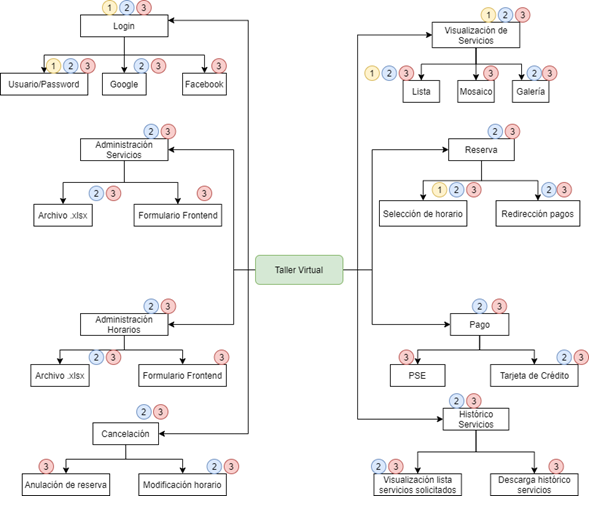
\includegraphics[width=1\textwidth]{img2}
	\caption{Taxonomía final de Talleres Automovilísticos Virtuales}
	\label{fig:img2}
\end{figure}


\begin{table}[htbp]
\centering
\begin{tabular}{|p{5cm}|p{3cm}|p{3cm}|p{3cm}|} \hline
Caracrteristicas descubiertas & Taller Virtual 1 & Taller Virtual 2 & Taller Virtual 3 \\ \hline
            C1 login                    & SI & \multirow{8}{3cm}{SI} & \multirow{8}{3cm}{SI}  \\
\cline{0-1} C2 Administración Servicios & NO & & \\
\cline{0-1} C3 Administración Horarios  & NO & & \\
\cline{0-1} C4 Cancelación              & NO & & \\
\cline{0-1} C5 Visualización Servicios  & SI & & \\
\cline{0-1} C6 Reserva                  & SI & & \\
\cline{0-1} C7 Pago                     & NO & & \\
\cline{0-1} C7 Historicos de Servicios  & NO & & \\\hline
\end{tabular}
\caption{Resumen de las características para los Talleres Virtuales }
\label{table:t9}
\end{table}

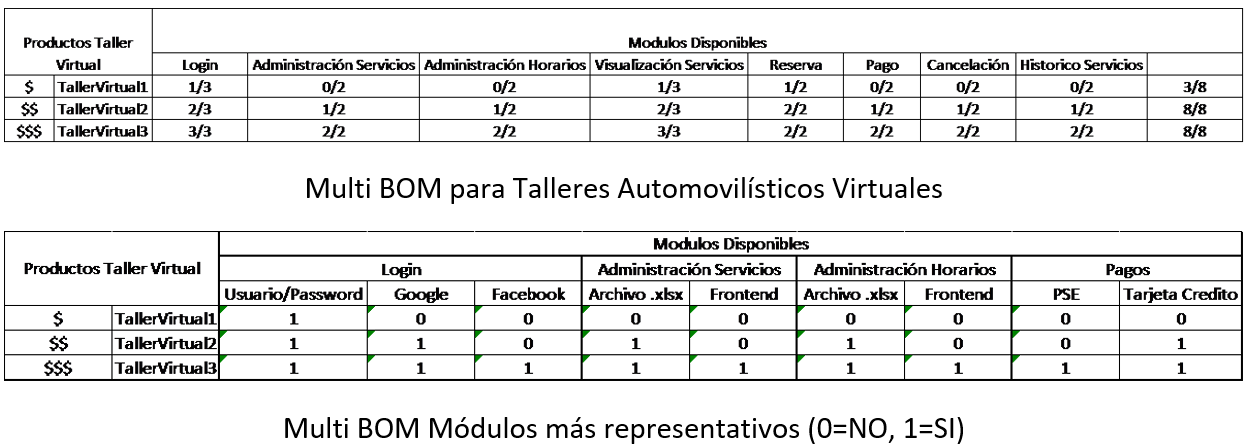
\includegraphics[width=1\textwidth]{t10}

%----------------------------------------------------------------------------------------
%	1.5 Evolución
%----------------------------------------------------------------------------------------
\section{Evolución}

Para la implementación de la LP se van a tener en cuenta los siguientes ambientes como se miestra en la Figura~\ref{fig:img1}, para soportar la evolución de la LPS y adaptarnos a cualquier cambio y funcionalidades nuevas que se deseen implementar:\\

\begin{figure}[h]
	\centering
	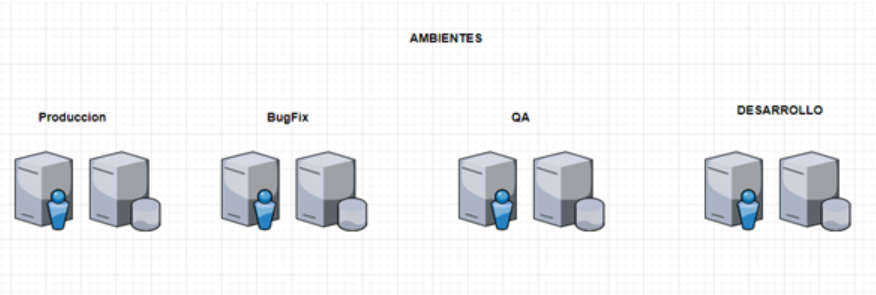
\includegraphics[width=1\textwidth]{img1}
	\caption{Diagrama ambientes de trabajo}
	\label{fig:img1}
\end{figure}

\begin{itemize}
	\item Producción: Tendrá la última versión estable de la LP y con las funcionalidades estables
	\item BugFix: Ambiente de donde se corrigen errores es muy cercano a producción para problemas que deben ser solucionados en corto tiempo.
	\item QA: Ambiente para los criterios de aceptación de desarrollos nuevos 
	\item Desarrollo: Ambiente para la integración de los desarrollos nuevos por cada programador
Para la implementación se manejar las siguientes tecnologías debido a que son muy estables además se cuenta con experiencia en el grupo implementador del LP y adicionalmente se estima que nos dará una estabilidad para 2 a 3 años para requerir una actualización necesaria:
	\begin{itemize}
		\item Postgres para base de datos
		\item HTML, JavaScript, JQuery, JSP, para el Frontend de la LP
		\item Framework PHP Laravel, Spring, para el Backend de la LP	
		\item Para el versionamiento se utilizará GIT
	\end{itemize}
	\item Las ramas para el versionamiento con git se proponen 4 ramas que serían:
	\begin{itemize}
		\item Master: Rama principal para desplegar el desarrollo estable y en producción
		\item Desarrollo: Rama para integración de nuevos desarrollos
		\item Release: Rama para tener nuevas funcionalidades y pruebas que no afecte producción	
		\item Bugfix: Rama sacada de Máster para corregir errores en producción
	\end{itemize}
\end{itemize}


%----------------------------------------------------------------------------------------
%	2 Espacio del problema
%----------------------------------------------------------------------------------------
\chapter{Espacio del problema}

\section{Ingeniería de requisitos del dominio}
Para la especificación de los requisitos utilizaremos el siguiente témplate

\begin{table}[htbp]
\centering
\begin{tabular}{|c|p{10cm}|} \hline
Nombre del atributo & Descripción \\[0.5ex] \hline
ID & Identificador único del requisito. la primera leta hace referencia al modulo al que pertenece (X) Todo el Sistema,(S) Servicios,(L) Login, (R) Reserva, (P) Pago, (A) Administración, la segunda letra hace referencia al tipo de requisito (F) Funcional, (N) No funcional, (C) Constraint, Ejemplo: PF\_1 = primer requisto funcional del modulo de pago \\[0.5ex] \hline
Modulo & Categoría a la que pertenece el requisito de acuerdo con el tema del proyecto y su funcionalidad.\\[0.5ex] \hline
Tipo & i el requisito es Funcional (RFU), si no es funcional (RNF) y si es una constraint (CON) \\[0.5ex] \hline
Version & En qué momento del desarrollo será llevada a cabo la realización del requisito.\\[0.5ex] \hline
Descripcion & Se detalla más a fondo el requisito.\\[0.5ex] \hline
Fuente & De donde se originó la idea del requisito: cliente, asesor, alguna técnica utilizada, etc.\\[0.5ex] \hline
Variablilidad & si el requisito va en core (False) y si es variable (True) \\[0.5ex] \hline
Estabilidad &  Que tan estable es el requisito para realizar cambios de (0-5) donde 0 no es estable y 5 es completamente estable\\[0.5ex] \hline
Fecha de entrega & La fecha de entrega del requisito a producción\\[0.5ex] \hline
Prioridad & (1-100) donde 100 es alta prioridad y 1 es baja prioridad\\[0.5ex] \hline
\end{tabular}
\caption{Témplate de Requisitos}
\label{table:t6}
\end{table}

\textbf{Palabras clave:}
\begin{itemize}
\item \textbf{Gestionar:} Realizar un CRUD crear editar eliminar  
\item \textbf{N/A:} No aplica 
\end{itemize}
\vspace{6cm}

\begin{longtable}{|p{1cm}|p{1cm}|p{1cm}|p{0.6cm}|p{4.4cm}|p{1.2cm}|p{0.8cm}|p{1cm}|p{2cm}|p{1cm}|} \hline

  {\rotatebox{90}{ID}} &
  {\rotatebox{90}{Modulo}} & 
  {\rotatebox{90}{Tipo}} & 
  {\rotatebox{90}{Version}} & 
  {\rotatebox{90}{Descripcion}} & 
  {\rotatebox{90}{Fuente}} & 
  {\rotatebox{90}{Variablilidad}} &
  {\rotatebox{90}{Estabilidad}} &
  {\rotatebox{90}{Fecha de entrega  }} &
  {\rotatebox{90}{Prioridad}}  \\[0.5ex] \hline
   
  AF\_1 &
  {\rotatebox{270}{ADMINISTRACIÓN }} & 
  RFU& 
  0.1 & 
  Los sistemas de Talleres WEB deberan proveer a los administradores la opcion de gestionar los servicios ofrecidos  & 
  William Garzon & 
  False &
  5 &
  15/12/2020 &
  100 \\[0.5ex] \hline
  
 
  
  AF\_2 &
  {\rotatebox{270}{ADMINISTRACIÓN }}  & 
  RFU& 
  0.1 & 
  Los sistemas de Talleres WEB deberan proveer a los administradores la opcion de gestionar los Horarios de atencion al publico  & 
  William Garzon & 
  False &
  5 &
  15/12/2020 &
  100 \\[0.5ex] \hline
  
  
  AF\_3 &
  {\rotatebox{270}{ADMINISTRACIÓN }}  & 
  RFU& 
  0.2 & 
  Los sistemas de Talleres WEB pueden proveer a los administradores genrerar el cobro a las reservas  & 
  William Garzon & 
  True &
  5 &
  29/01/2021 &
  1 \\[0.5ex] \hline
  
  
  AF\_4 &
  {\rotatebox{270}{ADMINISTRACIÓN }}  & 
  RFU& 
  0.1 & 
  Los sistemas de Talleres WEB deberán proveer a los administradores una Dashboard que les permita acceder al módulo de administración cuando el administrados haya iniciado sección & 
  William Garzon & 
  False &
  5 &
  15/12/2020 &
  100 \\[0.5ex] \hline
  
  AN\_5 &
  {\rotatebox{270}{ADMINISTRACIÓN }}  & 
  RFU& 
  0.2 & 
  Los sistemas de Talleres WEB deberán listar los servicios existentes al administrador en menos de 1 segundo & 
  William Garzon & 
  True &
  5 &
  29/01/2021 &
  1 \\[0.5ex] \hline
  
  
  XN\_3 &
  {\rotatebox{270}{TODOS }}  & 
  RFU& 
  0.1 & 
  Los sistemas de Talleres WEB deben customizar su interfaz según los estándares de cada cliente & 
  William Garzon & 
  True &
  0 &
  15/12/2020  &
  60 \\[0.5ex] \hline
  
  
  RF\_1 &
  {\rotatebox{270}{RESERVA }}  & 
  RFU& 
  0.1 & 
  La LP de Talleres WEB deberá permitir que en todo momento un usuario registrado pueda reservar un servicio. & 
  Dario Narváez & 
  False &
  5 &
  15/12/2020  &
  100 \\[0.5ex] \hline
  
  RF\_2 &
  {\rotatebox{270}{RESERVA }}  & 
  RFU& 
  0.1 & 
  La LP de Talleres WEB deberá permitir que en todo momento un usuario registrado pueda cancelar una reserva. & 
  Dario Narváez & 
  False &
  5 &
  15/12/2020  &
  100 \\[0.5ex] \hline

  RF\_3 &
  {\rotatebox{270}{RESERVA }}  & 
  RFU& 
  0.1 & 
  La LP de Talleres WEB deberá permitir que en todo momento un usuario registrado pueda modificar una reserva. & 
  Dario Narváez & 
  False &
  5 &
  15/12/2020  &
  100 \\[0.5ex] \hline 

  PF\_1 &
  {\rotatebox{270}{PAGO }}  & 
  RFU& 
  0.1 & 
  La LP de Talleres WEB deberá permitir que en todo momento un usuario registrado pueda realizar el pago de un cobro generado y que disponga de un medio de pago valido.  & 
  Dario Narváez & 
  False &
  5 &
  15/12/2020  &
  100 \\[0.5ex] \hline 

  PF\_2 &
  {\rotatebox{270}{PAGO }}  & 
  RFU& 
  0.1 & 
  La LP de Talleres WEB debe tener en su componente de pago la opción de pago en efectivo. & 
  Dario Narváez & 
  False &
  5 &
  15/12/2020  &
  100 \\[0.5ex] \hline 
  
  PF\_3 &
  {\rotatebox{270}{PAGO }}  & 
  RFU& 
  0.1 & 
  La LP de Talleres WEB puede tener en su componente de pago las siguientes opciones de pago: PSE o tarjeta crédito.
 & 
  Dario Narváez & 
  True &
  5 &
  15/12/2020  &
  100 \\[0.5ex] \hline 

   &
   & 
   & 
   & 
   & 
   & 
   &
   &
   &
   \\[0.5ex] \hline
  

\caption{Requisitos}
\label{table:t5}
\end{longtable}

\section{Modelo de variablilidad}

\begin{figure}[h]
	\centering
	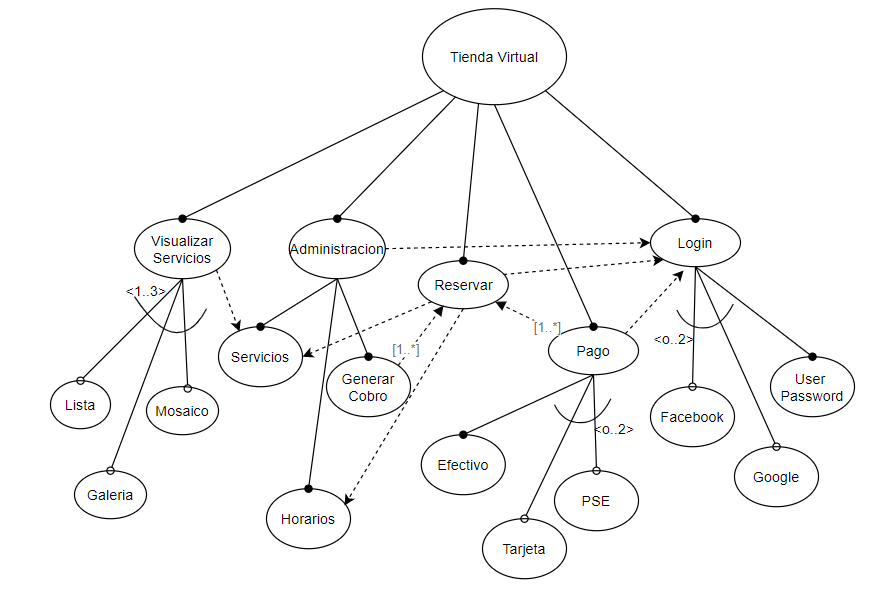
\includegraphics[width=1\textwidth]{img3}
	\caption{Modelo de Variablilidad}
	\label{fig:img3}
\end{figure} 


\section{Diagnóstico y reparación del modelo de Variablilidad}
Para realizar el diagnóstico y reparar nuestro modelo de variabilidad transformaremos el modelo en lenguaje GNU prolog.\\
\begin{figure}[h]
	\centering
	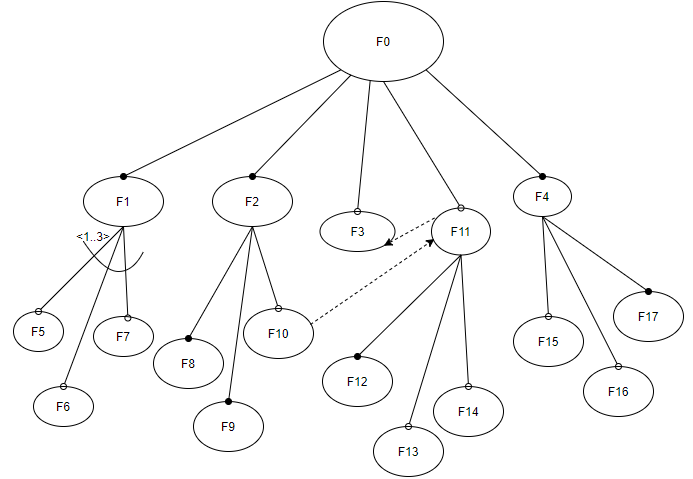
\includegraphics[width=0.8\textwidth]{img4}
	\caption{Modelo de Variablilidad de referencia para GNU prolog}
	\label{fig:img4}
\end{figure} 

\begin{figure}[h]
	\centering
	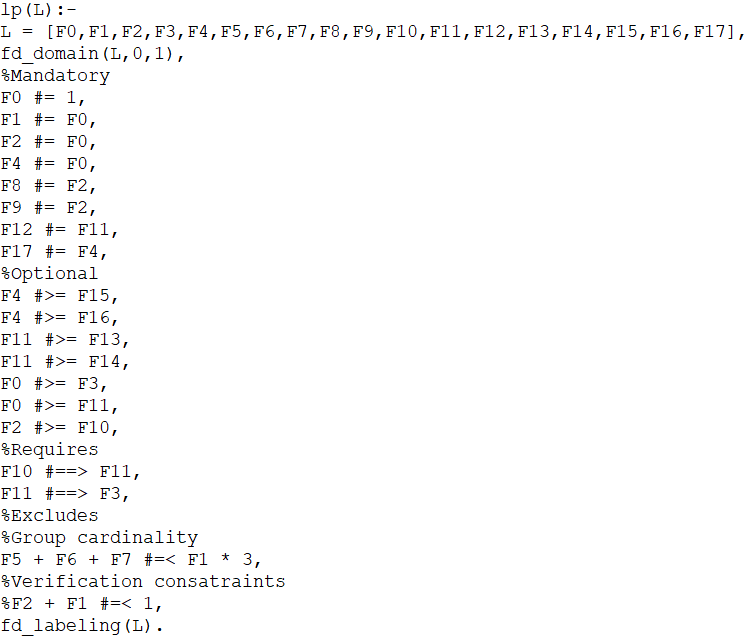
\includegraphics[width=1\textwidth]{gnu}
	\caption{Modelo de Variablilidad en lenguaje GNU prolog}
	\label{fig:gnu}
\end{figure} 

\begin{figure}[h]
	\centering
	\caption{findall(Config,lp(Config),Solutions), length(Solutions,Nsolutions).}
	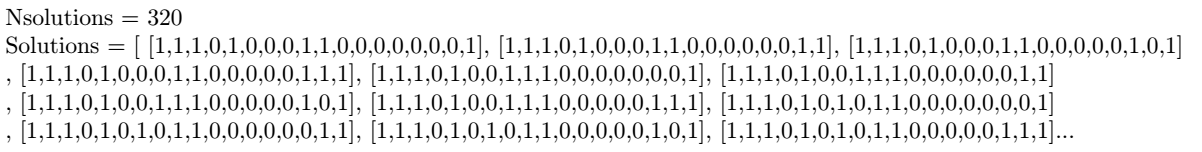
\includegraphics[width=1\textwidth]{gnu1}
	\label{fig:gnu1}
\end{figure}

\begin{figure}[h]
	\centering
	\caption{Algunas validaciones del modelo.}
	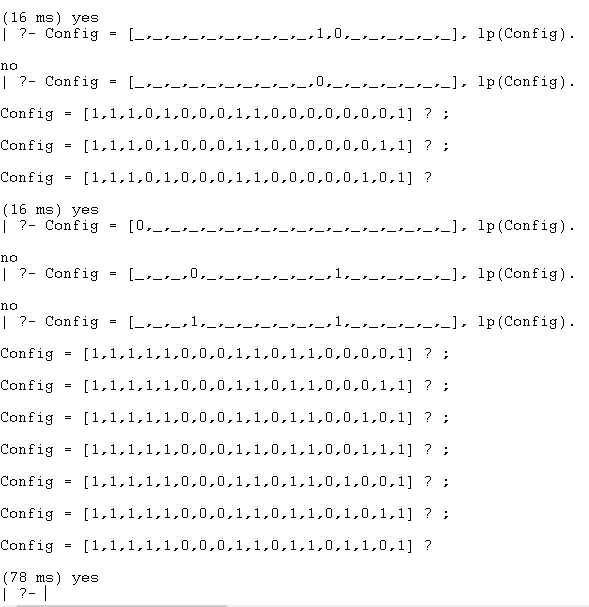
\includegraphics[width=1\textwidth]{gnu2}
	\label{fig:gnu2}
\end{figure}



%----------------------------------------------------------------------------------------
%	3 Definición de la arquitectura de referencia del dominio
%----------------------------------------------------------------------------------------
\chapter{Definición de la arquitectura de referencia del dominio}

\section{Construir el modelo de variabilidad}
\subsection{Identificar la variabilidad en los tipos de aplicación}
La LP de Talleres WEB no requiere características complejas, ni tampoco una interfaz de usuario rica en gráficos. Pero, si requiere independencia del lado del cliente, simplicidad y accesibilidad desde Internet. También, la LP de Talleres WEB podrá a futuro exponer funcionalidades para que puedan ser consumidas por aplicaciones para la reserva de servicios de talleres automovilísticos.\\

Basados en lo anterior la LP de Talleres Web deberá soportar: Aplicaciones Web y Aplicaciones Orientadas a Servicios.


\subsection{Identificar la variabilidad en el estilo arquitectónico}
Estilos de arquitecrura considerados \cite{url3}


\begin{enumerate}
\item Web Application
\begin{itemize}
	\item Utilizar capas para dividir la aplicación de manera lógica en capas de presentación, negocios y acceso a datos. Ayuda a crear código mantenible y nos permite monitorear y optimizar el rendimiento de cada capa por separado.\\\\
Utilizar la abstracción para implementar un acoplamiento flexible entre capas mediante la definición de componentes de interfaz, como una fachada con entradas y salida.\\\\
Considere el almacenamiento en caché para minimizar los viajes de ida y vuelta del servidor.
\end{itemize}
\begin{center}
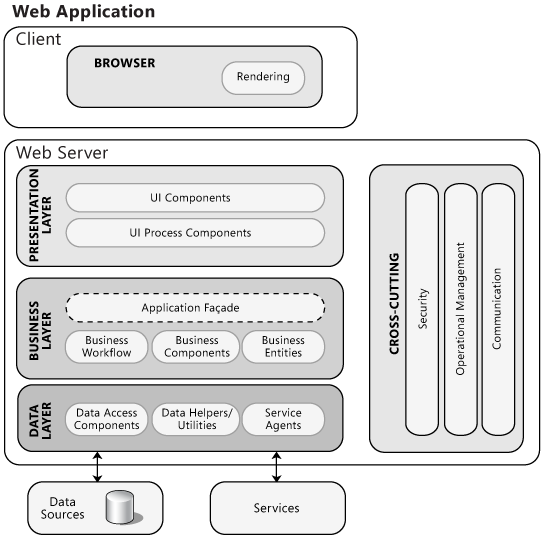
\includegraphics[width=0.5\textwidth]{arq1}
\end{center}
\item Service Applications
\begin{itemize}
	\item Utilizar una interfaz pública que proporciona acceso a una unidad de funcionalidad mediante servicios expuestos a travéz de internet y que están débilmente acoplados y pueden combinarse dentro de un cliente, o combinarse con otros servicios, para proporcionar una funcionalidad que es más compleja.\\\\
	Considerando el uso de un enfoque por capas para diseñar aplicaciones de servicio y evitar el acoplamiento estrecho entre capas.\\\\
	Asegurando la autentificación mediante web token el cual nos permite gestionar de manera eficiente nuestra LP, otorgando accesos definidos por cada perfil del aplicativo.
\end{itemize}
\begin{center}
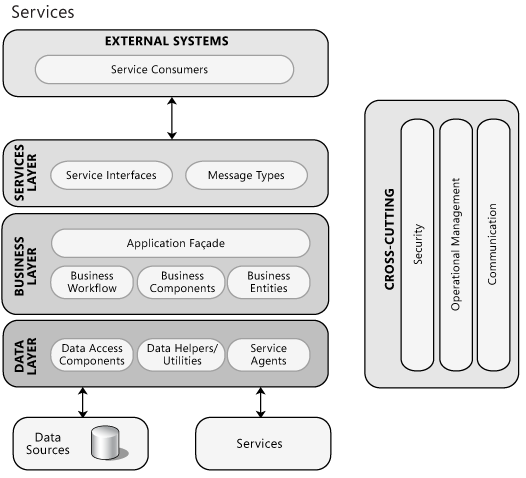
\includegraphics[width=0.5\textwidth]{arq2}
\end{center}
\end{enumerate}



\subsection{Identificar la variabilidad en las estrategias de despliegue}
\subsection{Identificar la variabilidad en los aspectos técnicos}
\subsection{Modelo de variabilidad de la arquitectura de referencia}
\begin{center}
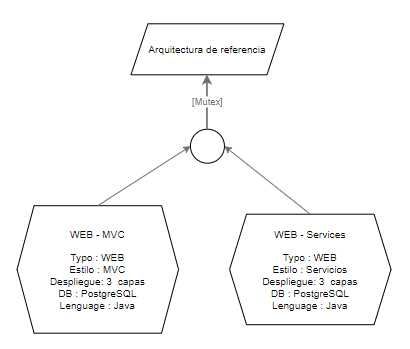
\includegraphics[width=0.5\textwidth]{model1}\\
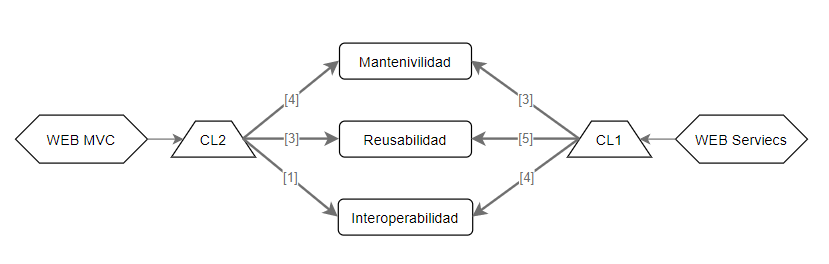
\includegraphics[width=0.8\textwidth]{model2}
\end{center}

\subsection{referencia resultante arquitectura}
\subsubsection{Diseño de la Arquitectura de referencia}
\begin{center}
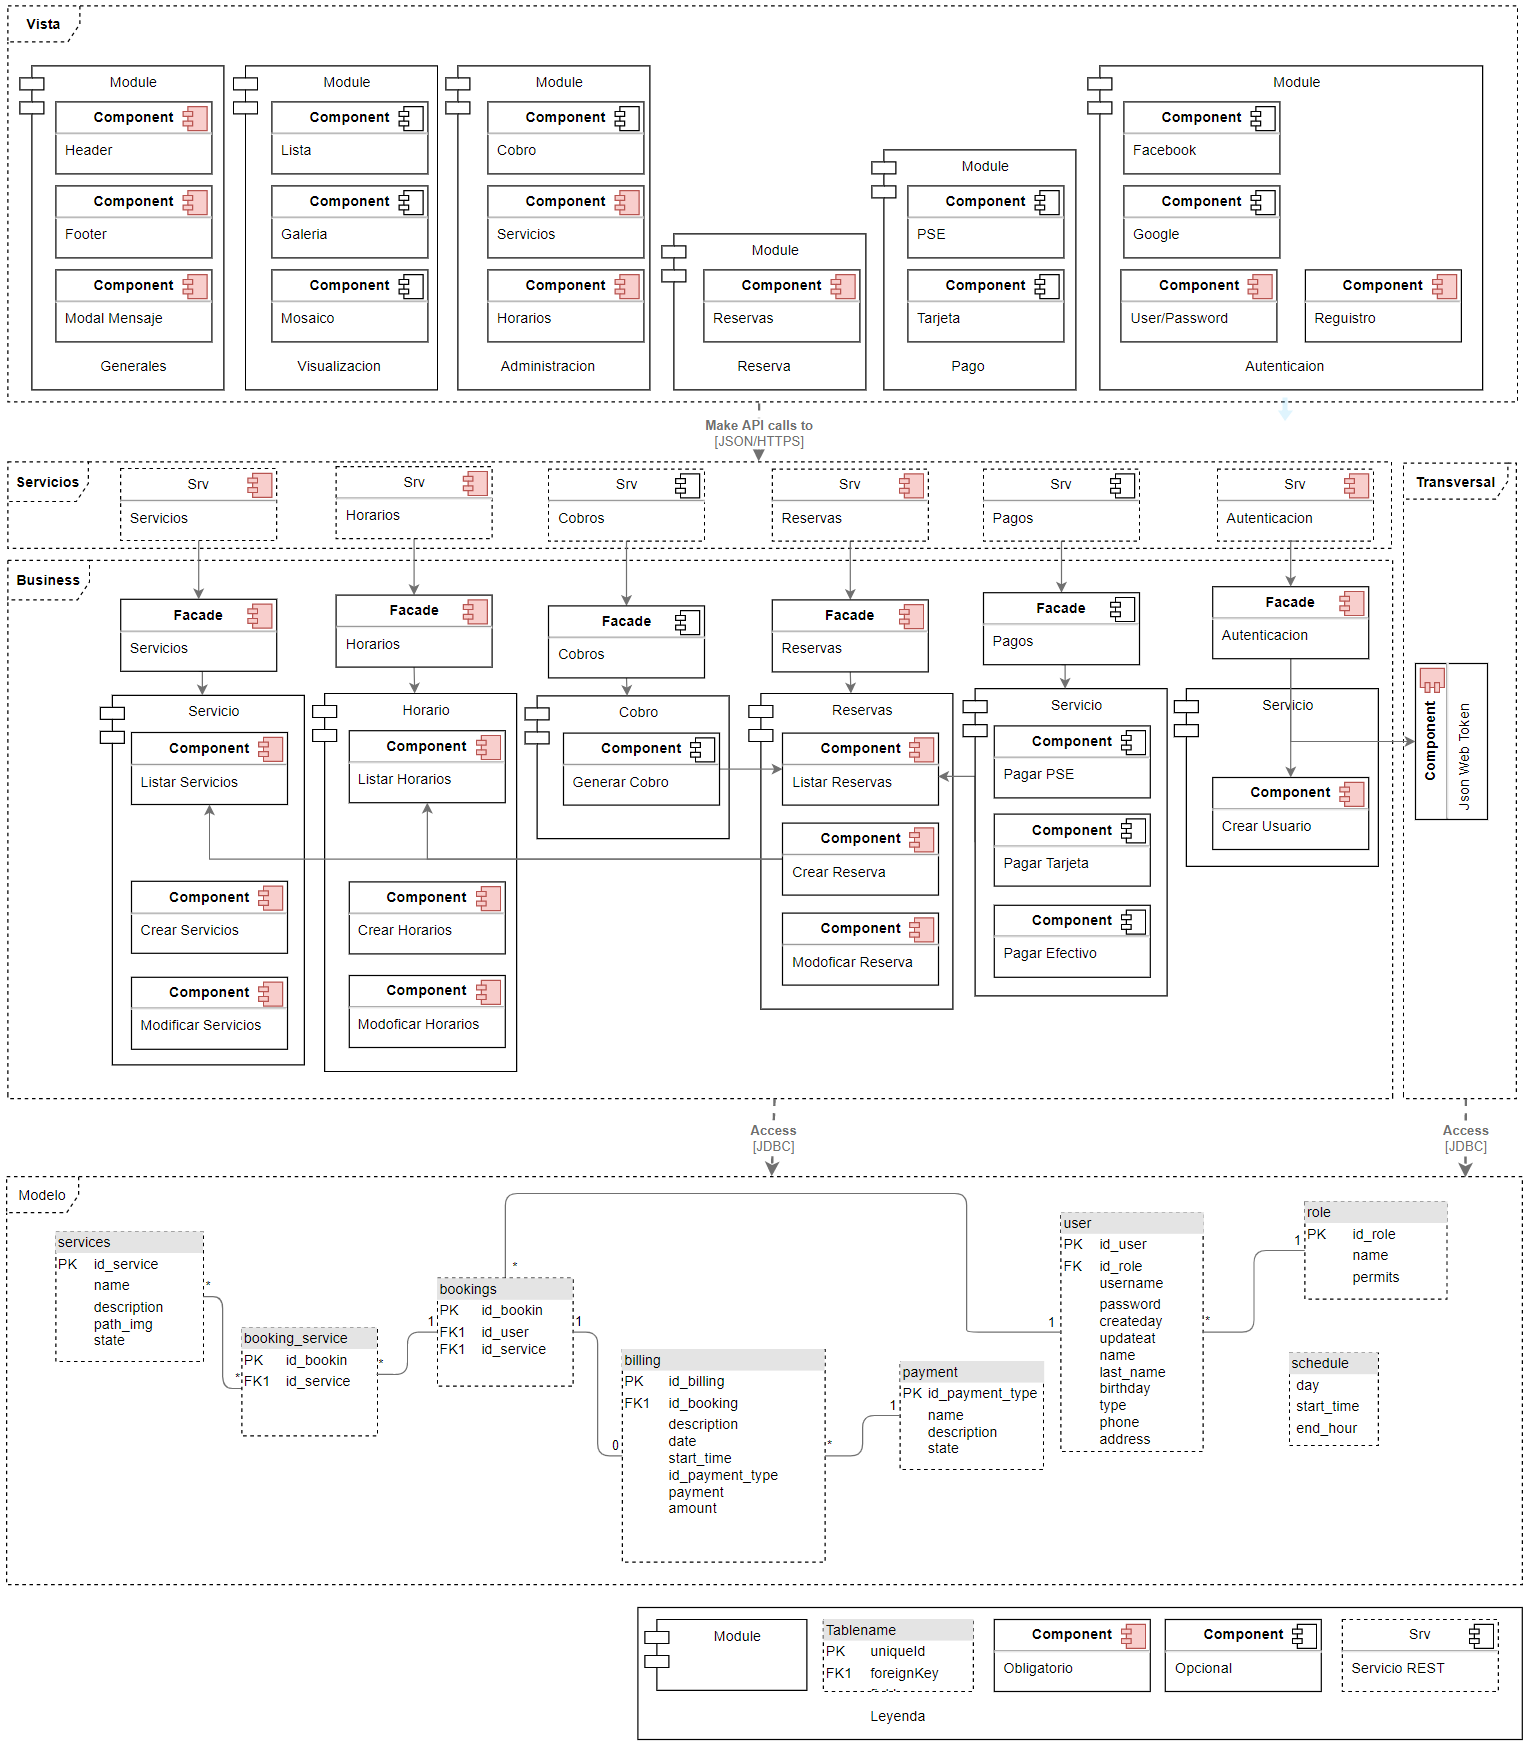
\includegraphics[width=0.8\textwidth]{arq3}
\end{center}

\subsubsection{Documentación de componentes de dominio a nivel de diseño}
\begin{center}
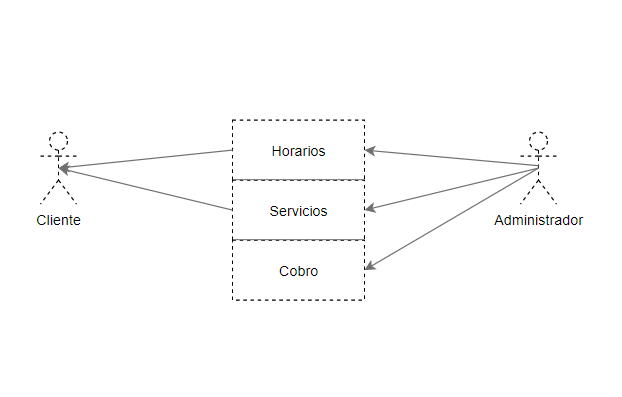
\includegraphics[width=0.8\textwidth]{dominio}
\end{center}

\subsubsection{Documentación general del componente }

\begin{longtable}{|p{3cm}|p{3cm}|p{3cm}|p{3cm}|p{3cm}|} \hline
Identificación & Nombre del componente & Administración de categorías & Identificador del componente & AdCategorías \\[0.5ex] \hline
& & & & \\[0.5ex] \hline
Gestión variabilidad componente & \multicolumn{4}{|c|}{Define si el componenete es común para cualquier linea de producto} \\ \hline
Tipo de componente & \multicolumn{4}{|c|}{Define si es desarrollo es propio o es tercerisado} \\ \hline
Resumen del componente & \multicolumn{4}{|c|}{Para que sirve el componente} \\ \hline
Requisistos que implementa el componenete & \multicolumn{4}{|c|}{Requisitos realcionados con las categorías asociadas a los productos } \\ \hline
Versión & \multicolumn{4}{|c|}{ numero de version } \\ \hline
Fecha revisión & \multicolumn{4}{|c|}{ Fecha del diseño:} \\ \hline
Diseño & \multicolumn{4}{|c|}{Quien realizo el diseño} \\ \hline
Desarrolladores & \multicolumn{4}{|c|}{Por definir} \\ \hline
Decisiones técnicas & \multicolumn{4}{|c|}{Anotaciones tecnicas del componente} \\ \hline
Restricciones & \multicolumn{4}{|c|}{De dsiponibilidad} \\ \hline
Atributos de calidad & \multicolumn{4}{|c|}{Atributos asociados al componente} \\ \hline
\caption{Témplate para documentar componentes}
\label{table:t6}
\end{longtable}




\medskip
\bibliographystyle{abbrv}
\bibliography{libreria}
\end{document}
